\documentclass[12pt]{article}
%\usepackage{tkiz}

\usepackage[utf8]{inputenc}
\usepackage[french]{babel}
\usepackage{amsmath,amsthm,amsfonts,amssymb}
\usepackage{lmodern}
\usepackage[top=2.4cm,bottom=2.4cm,left=2cm,right=2cm]{geometry}
\usepackage{hyperref}
\usepackage{multicol}
\usepackage{enumitem}
\usepackage{listings}
\usepackage[dvipsnames]{xcolor}
\usepackage{tikz}

%\date{}
\title{{\bf  Génie logiciel} \\
	Notes du cours de 21/10 , partie 1 \\
	{\small L3 Informatique appliquée 2022-2023} \\
	{\it \small MABROUK Fayez}}
\begin{document}
	\maketitle
	\newpage
	\section{Diagrammes de cas d'utilisation}
	\subsection{Relations entre les cas d'utilisation - Inclusion}
	\begin{itemize}
		\begin{figure}[!hbtp]
			%\centering
			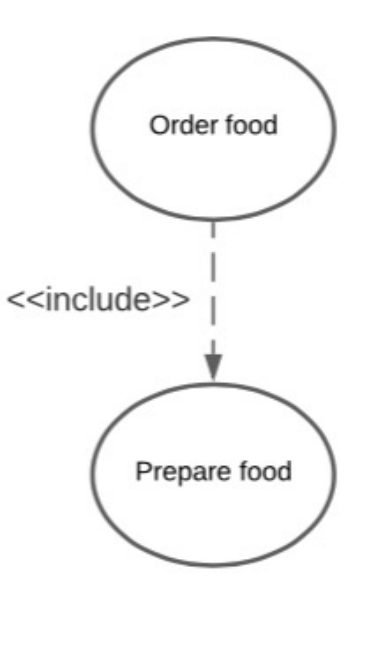
\includegraphics[scale=0.75]{Capture.PNG}
			%\caption{Légende de l'image}
		\end{figure}
		\item [*] Jusqu'à présent, nous avons vu les acteurs, les cas d'utilisation et les relations
		entre eux.
		\item [*] Il est également possible d'avoir des relations entre les cas d'utilisation.
		\item [*] Relation d'inclusion.
		\item[*] représentée par une flèche en pointillés avec la spécialisation
		<<include>>.
		\item [*] Peut décrire une sous-fonctionnalité.
		\item [*] Ou peut être utilisée pour partager des fonctionnalités.
		\item [*] Doit toujours être exécutée.
		\item [*] Ne répond pas directement à un objectif de l'acteur primaire.
	\end{itemize}
\subsection{Relations entre les cas d'utilisation - Extension}
\begin{itemize}
	\newpage
		\begin{figure}[!hbtp]
			%\centering
			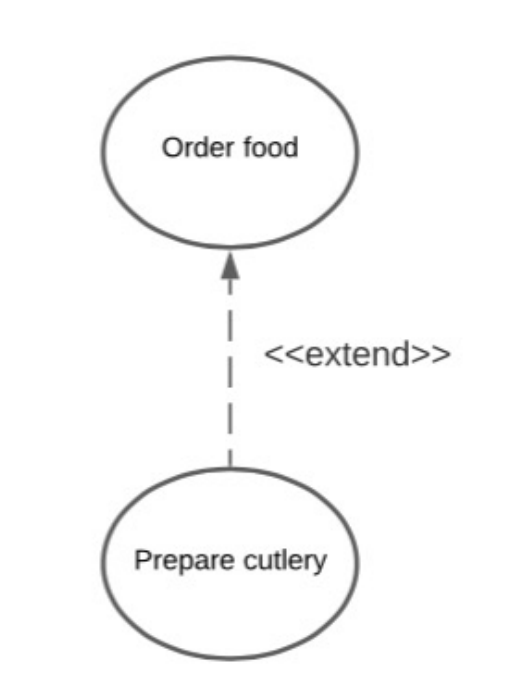
\includegraphics[scale=0.75]{Capture1.PNG}
			%\caption{Légende de l'image}
		\end{figure}
		\item [*] Extension : similaire à l'inclusion, mais
		facultative.
		\item[*] L'application d'une extension est décidée
		au cours du scénario.
		\item[*] Représentée par une flèche en pointillés avec
		la spécialisation <<extend>>.
	\end{itemize}
\subsection{Relations entre les cas d'utilisation}
\begin{itemize}
	\item [*] Spécialisation : comme pour les classes.
	\item[*] Donne un sous-cas d'utilisation
	\item [*] Permet d'hériter du comportement, des
	associations aux acteurs et aux cas d'utilisation.
	\item [*] Le cas d'utilisation à partir duquel il se généralise est souvent
	abstrait. Dans ce cas, le nom est en
	italique.
	\item [*] Représentation : flèche blanche.
	\begin{figure}[!hbtp]
		%\centering
		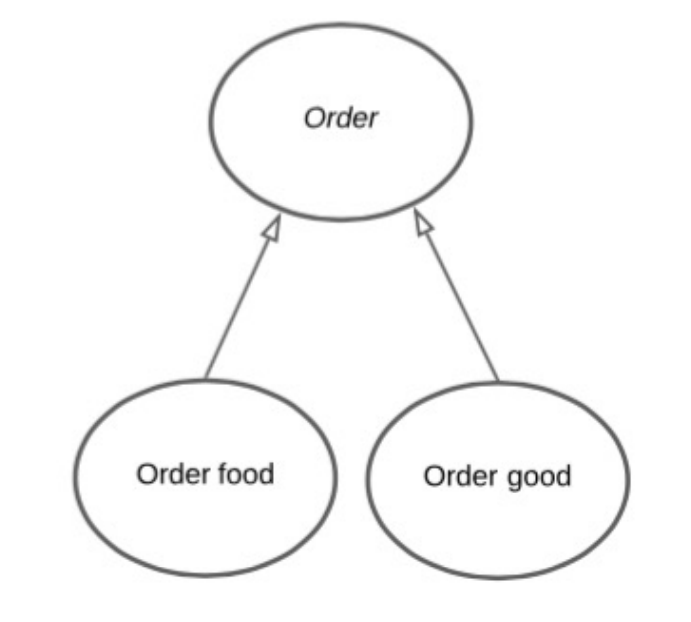
\includegraphics[scale=0.75]{Capture2.PNG}
		%\caption{Légende de l'image}
	\end{figure}
\end{itemize}
\subsection{Comment représenter un cas d'utilisation ?}
\begin{itemize}
	\item [*] Le diagramme de cas d'utilisation est essentiel à la représentation d'un cas d'utilisation, mais pas suffisant.
	\item[*] Doit être accompagné d'un document précisant :
	\begin{itemize}
		\item[*] Acteur principal.
		\item [*] Acteurs secondaires (facultatif).
		\item[*] Quel système.
		\item[*] Niveau du cas d'utilisation (objectif principal pour l'acteur principal, ou sous-fonction ?).
		\item [*] le glossaire.
		\item [*] Hypothèses (qui sont supposées vraies pour une exécution correcte).
		\item [*] Cas d'utilisation alternatifs.
		\item[*] Extensions du cas d'utilisation.
		\item[*] Et les informations habituelles (Nom, date, version, ...).
	\end{itemize}
\end{itemize}
\subsection{Conclusion}
\begin{itemize}
	\item [*] Les cas d'utilisation permettent :
	\begin{itemize}
		\item[*] De recueillir les exigences fonctionnelles.
		\item [*] D'analyser les besoins fonctionnels.
		\item[*] De discuter des exigences fonctionnelles.
		
	\end{itemize}
\item[*]  Ils permettent de comprendre les limites du système.
\item [*] Ils peuvent être utilisés pour concevoir les interfaces du système.
\item[*] Il permet de valider les exigences.
\item[*] Il peut faire partie de la documentation.
\item[*] ATTENTION : il ne s'agit pas d'un diagramme temporel... Semaine prochaine !
\end{itemize}
\end{document}